
\section*{RUP: Rational Unified Process}

La metodología utilizada para la elaboración de este proyecto ha sido 
\emph{RUP}\footnote{\url{http://www.rational.com/products/rup/}}
(Rational Unified Process, Proceso Racional Unificado) de IBM.

La razón principal fue la genericidad que brinda para el proceso de desarrollo
software, adaptandose perfectamente a desarrollos basados en programación 
orientada a objetos.

Ayudo a implementar determinadas buenas prácticas en Ingeniería del Software:

\begin{itemize}
  \item Desarrollo iterativo
  \item Administración de requisitos
  \item Uso de arquitectura basada en componentes
  \item Control de cambios
  \item Verificación de la calidad del software
\end{itemize}

Por tanto todo el proceso de desarrollo se dividió en ciclos, teniendo un 
producto final al final de cada ciclo, dividiendo cada ciclo en fases que 
finalizan con un hito importante.

\begin{figure}[ht]
	\centering
	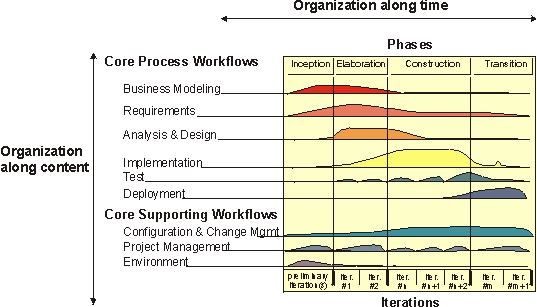
\includegraphics[width=12cm]{images/rup.png}
	\caption{Vista general de RUP}
	\label{fig:RUP}
\end{figure}

Los fases seguidas fueron:

\begin{enumerate}
  \item Inicio: se hizo un plan de fases, identificando los principales 
	casos de uso y riesgos.
  \item Elaboración: se hizo un plan de proyecto, completandose los casos 
	de uso para eliminar los riesgos.
  \item Construcción: se concentro en la elaboración de un producto totalmente 
	operativo y eficiente, asicomo en un pequeño manual de usuario.
  \item Transición: se implemento el producto en el cliente y se publicaron
	varias versiones funcionales. Como consecuencia de esta publicación
	surgieron nuevos requisitos a ser analizados.
\end{enumerate}

Para cada fase RUP define nueve actividades a realizar:

\begin{enumerate}
 \item Modelado del negocio
 \item Análisis de requisitos
 \item Análisis y diseño
 \item Implementación
 \item Test
 \item Distribución
 \item Gestión de configuración y cambios
 \item Gestión del proyecto
 \item Gestión del entorno
\end{enumerate}

Además de un flujo de trabajo entre ellas:

\begin{figure}[ht]
	\centering
	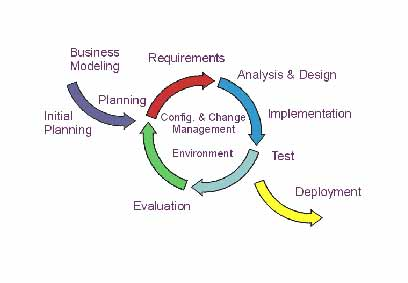
\includegraphics[width=9cm]{images/workflow-rup.png}
	\caption{Flujos de trabajo de RUP}
	\label{fig:RUP}
\end{figure}

En RUP de utiliza UML\footnote{\url{http://www.omg.org/uml/}} como herramienta principal
para la documentación de toda la arquitectura del sistema. La bibliografia es amplia,
disponiendo de veteranos títulos como 
\emph{The Unified Modeling Language Reference Manual}\cite{UMLReference} o 
\emph{UML Distilled}\cite{UMLDistilled} como guias de referencia, siendo imprescidible
tener siempre a mano el \emph{UML 2.0 Pocket Reference}\cite{UMLPocket} para resolver
rápidamente esas consultas puntuales de la especificación.

RUP puede englobarse dentro de lo que algunos llaman \emph{procesos pesados},
estando quizás muy orientado para proyecto de algo más de envergadura que SWAML.
Es por ello que debido a las caracteristicas del proyecto, tamaño y personas 
involucradas, se ha adaptado RUP utilizando sólo los documentos y procesos de 
diseños necesarios.

Este método es de sobra conocido y esta perfectamente documentado (en libros como
\emph{The Rational Unified Process}\cite{RUPIntro} y
\emph{The Rational Unified Process Made Easy}\cite{RUPEasy}) como para
extenderse más reescribiendo dicha documentación.
